\chapter{}

\section{Abstract}

\section{Introduction}

With the development of neovel sequencing technologies, the price to sequence a single microbial genome has decreased considerable over the last years \cite{Mardis:2013gn}, increasing the number of microbial genomes in databases, helping investigation of comparative genomics, etc, etc. (REFs). 

Whole genome analysis allows to increase phylogenetic resolution among multiple groups, and also to start asking questions about the particular genomic features that affect the adaptation of each organism to the environment.

Now is possible to move from comparing a single genome to several (REFs)

Multiple databases exist where genomes have been compared and the data is already available in pre-calculated databases (REFs), but in some cases it is difficult to add or analyze recent genomes. A recent software ITEP, allows these comparasions. PSP allows also this, but is a web server

Selection analysis are important, not only gene content (absecnce presence)

In this chapter, I describe a pipeline developed for the comparative analysis of microbial genomes, with an emphasis on pan-genome anlaysis and selection analysis. All of the code is freely available in Github (link), and is currently being updated to be applied to large scale comparisons (~100 genomes).

\section{Overview of the analysis workflow}

The analysis strategy consists on several Python scripts that carry out the different steps of data analysis (Figure \ref{CompGenomePipeline}). All of the scripts are available in a public repository on Github (\url{http://github.com/juanu/CompMicroGenom}). The analysis steps can be summarized as:

\begin{itemize}
\item Data preprocessing
\item Ortholog search
\item Analysis of ortholog data
\item Selection analysis
\item Result summary
\end{itemize}

In the following sections, each of these steps will be explained in more detail.

\begin{figure}[htbp]
	\centering
	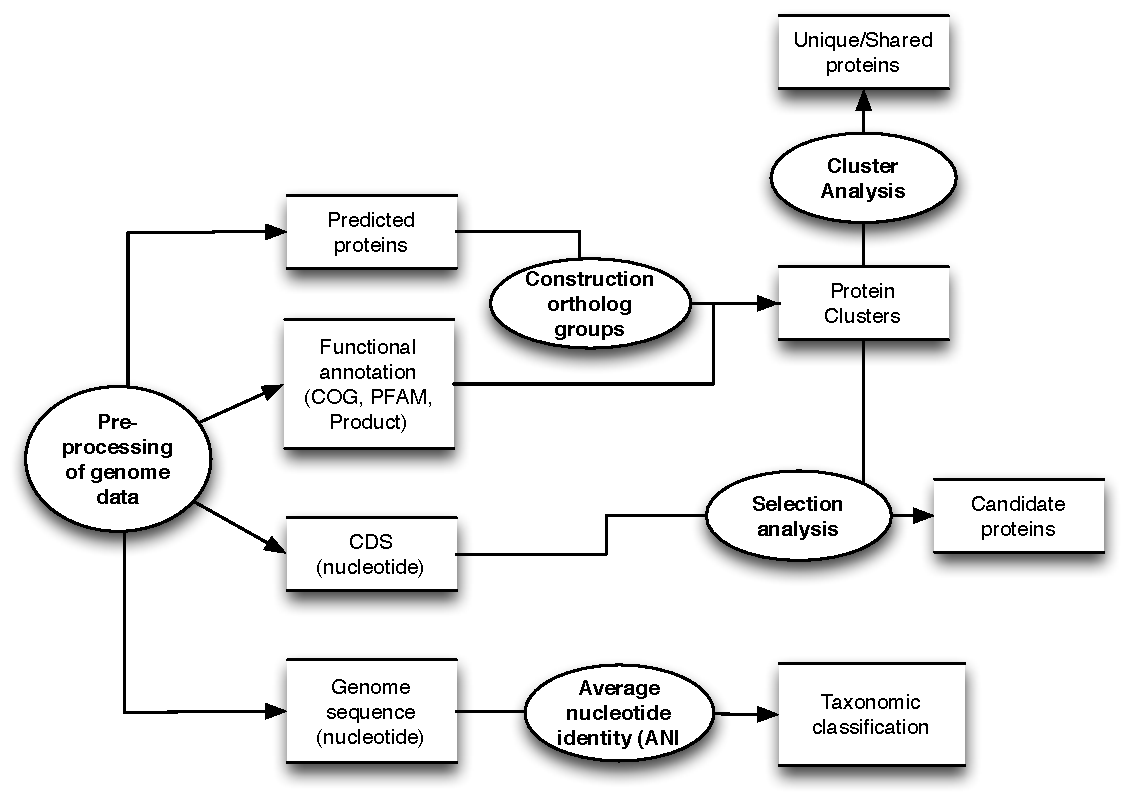
\includegraphics[width=\textwidth]{Chapter6/Figures/WorkflowOverview.pdf}
	\caption[Overview of the pipeline developed for the comparative analysis of microbial genomes]{Overview of the pipeline developed for the comparative analysis of microbial genomes.}
	\label{CompGenomePipeline}
\end{figure}

\subsection{Data preprocessing}

Several public resources are available for genome annotation and as repositories. Among some of the most used ones are the Integrated Microbial Genomes database\cite{Markowitz:2011ck}, NCBI and RAST \cite{Aziz:2008ku}. Although some of these repositories overlap in their content (in particular IMG and NCBI), the increase in the rates of submission of newer genomes, makes IMG slightly outdated in comparison to other resources. On the other hand, some of the genomes that are present on IMG are not available on NCBI and/or RAST. To be able to exploit all these available information, a pre-processing step is incorportated in the analysis to parse genomes obtained from these different sources, and put them into a common format that can be easily used through all the workflow (Figure \ref{Preprocessing}). Using this strategy, also allows to incorporate genomes from newer sources, by just adding a new parsing script. For example, it could be relatively easy to incorporate an in-house sequenced genome into this workflow, by using a genome annotation pipeline like Prokka \cite{Seemann:2014ks}, and connecting into this workflow.

\begin{figure}[htbp]
	\centering
	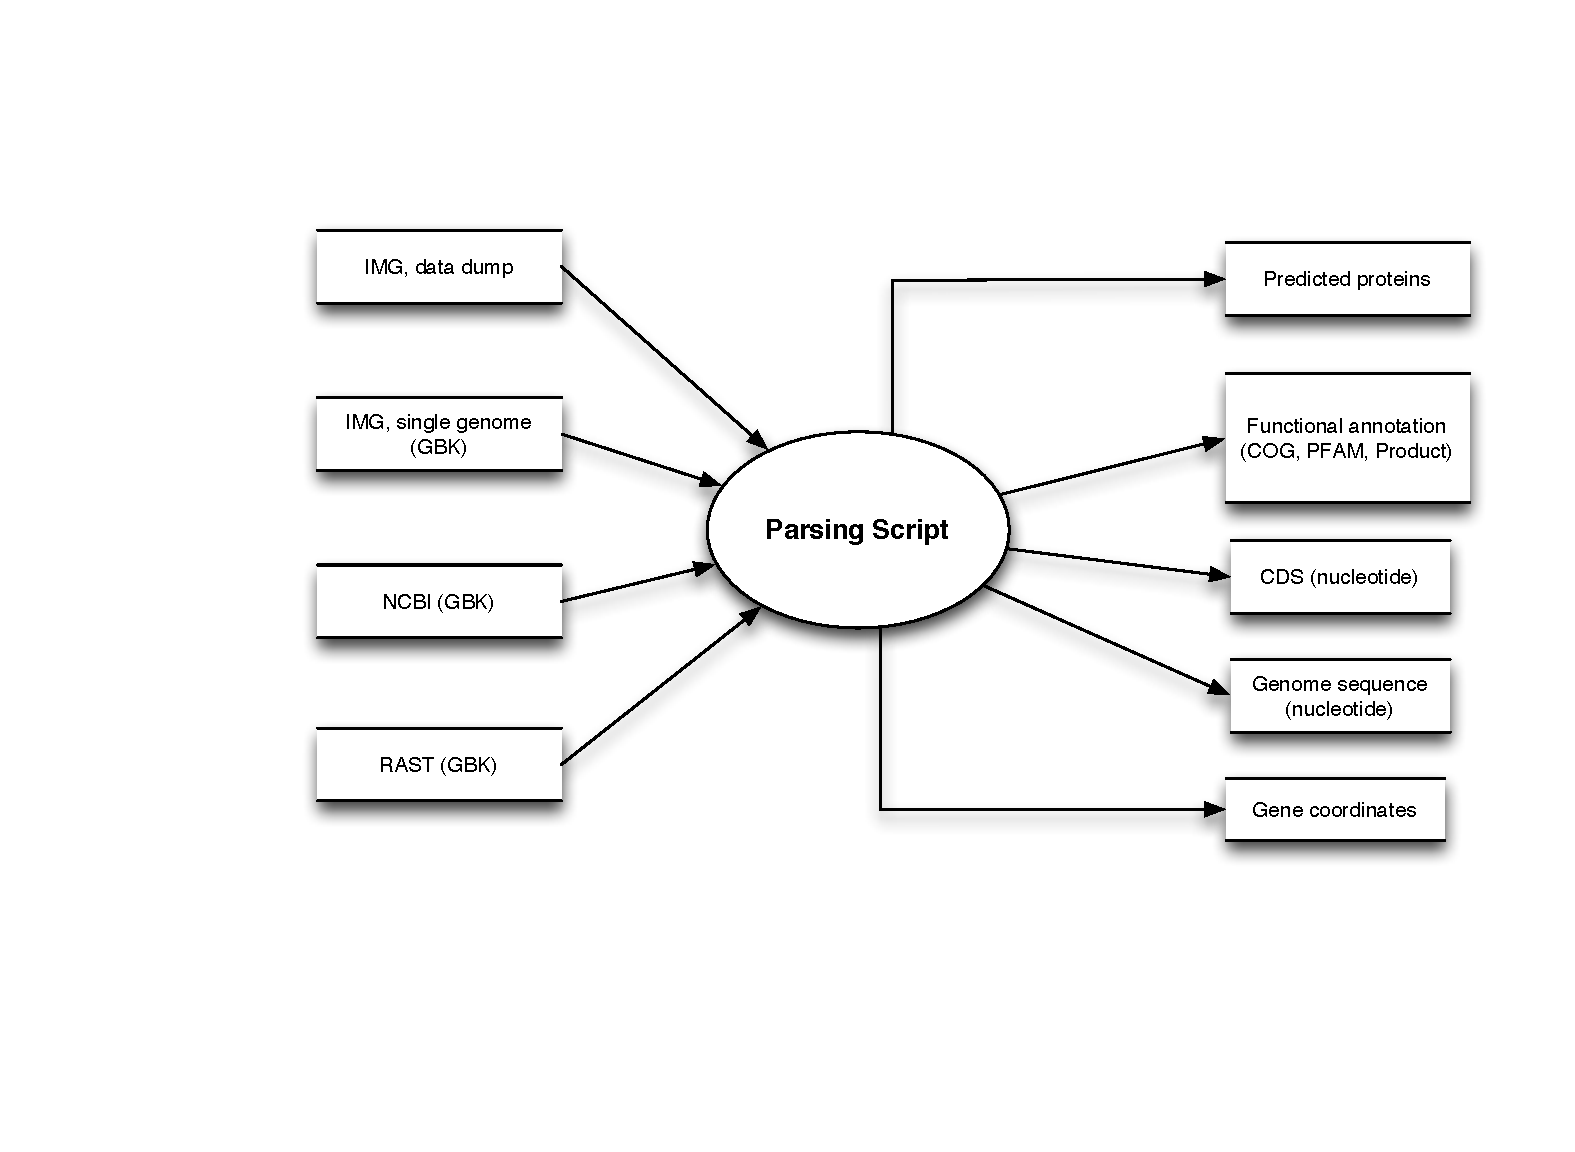
\includegraphics[width=\textwidth]{Chapter6/Figures/PreprocessingOverview.pdf}
	\caption{Preprocessing step}
	\label{Preprocessing}
\end{figure}

\subsection{Construction of orthologous groups}

The basis of this comparative genomic approach is the construction of orthologous groups of genes, a collection of all the descendants of an ancestral gene that diverged after a given speciation event  \cite{Kristensen:2011gw}. These groups provide us with a picture of the evolutionary history of the gene family (and its host organisms), and can be used for further studies on the basis for molecular adaptation of its host organisms.
Several approaches exists for the construction of ortholog groups \cite{Kristensen:2011gw}, which can be broadly classified in two categories: tree-based and heuristic based approaches. Tree based methods are computationally expensive and require a known phylogenetic relationship for the studied organisms, something that sometimes is difficult to generate in light of the presence of horizontal gene transfer events in microbial genomes \cite{Koonin:2001vz}. On the other hand, heuristic based approaches are easy to automatize and several implementations of these methods are already available \cite{Kristensen:2011gw}. Among the main drawbacks, the generated group of sequences may not reflect the true evolutionary history of the gene, specially in large and complicated protein families \cite{Chen:2007kk}.
In consideration of this evidence, we choose an heuristic-based approach to generate orthologous groups, because it can be easily scalable to hundreds of genome, and its easiness to incorporate into an automatic pipeline. OrthoMCL \cite{Li:2003en}, performs a bidirectional best hit search in the aminoacid space, using a "all-vs-all" blastp (although, other search methods could be implemented), followed by a subsequent clustering of the results using a Markov Clustering procedure \cite{Enright:2002uq}.

Within the current workflow, the construction of ortholog groups is based on the OrthoMCL protocol \cite{Li:2003en}, consisting of the following steps: 
\begin{itemize}
\item Protein blast of "all-vs-all" the proteins
	\begin{itemize}
	\item Concatenate all the protein sequences for the genomes of interest
	\item Create a Blast database
	\item Protein blast using these parameters: \textit{-F 'm S' -v 1000000 -b 1000000 -m 8}
	\end{itemize}
\item OrthoMCL analysis
	\begin{itemize}
	\item Create a MySQL database to store the OrthoMCL results
	\item Run OrthoMCL to generate a list containing pairs of sequences and their similarity score
	\item Use MCL to create clusters based on the previous results. Different inflation values can be tested, where smaller values give larger clusters.
	\end{itemize}
\end{itemize}

\subsection{Analysis of ortholog groups}

The clusters of sequences obtained from the previous step are processed using a set of Python scripts to summarize the results. Some of the information obtained here includes:

\begin{itemize}
\item List and count of unique sequences in each analyzed genomes
\item A list and count of single copy clusters; sequences that are present in single copy in all the analyzed genomes. 
\item A list and count of shared multiple copy clusters; sequences present in all the analyzed genomes, but that in some of them are present in more than one copy.
\end{itemize} 

Levering on these cluster results, several analysis can be performed using this information:

\subsubsection{Functional annotation}

The resulting protein clusters can be annotated, based on the information obtained from the annotation files. Currently the annotation incorporates information such as Cluster of Orthologous Groups (COGs), KEGG (REF) and PFAM domains (REF). The current approach for the annotation is to use a majority rule for the cluster, where each cluster is annotated with the function that half plus one of the proteins in the cluster have. This also serves as a validation step, because in classifications such as COGs, is expected that all of the members from the cluster should have the same COG number. Conflicts are recorded for validation as well.

\subsubsection{Alignment and tree construction}

As part of the pipeline, it is possible to generate alignments and trees for all (or a subset) of the clusters generated. The approach used is to generate an alignment of each cluster using MAFFT on the amino acid sequences, followed by a construction of a phylogenetic tree using FastTree. DNA alignments are generated by replacing each amino acid in the aligned sequences, with its corresponding codon from the DNA sequences, allowing for better DNA alignments. All of the resulting sequences (aligned and unaligned) are saved for future reference.

\subsubsection{Phylogenomic analysis}

One of the most important goals of the workflow is to generate information useful for phylogenomic analysis. Phylogenetic classification based on 16S rRNA sequences, lathough highly used, are limited by the sequence space of the 16S rRNA gene. Even species with highly similar 16S rRNA sequences, show differences both in their gene content and the functional capabilities. The use of marker genes, multi-locus sequence typing (MLST) and whole genome analysis, allow to increase the information and therefore the resolution of phylogenetic classifications. 

Within the scope of the workflow, the idea is to be able to identify clusters that are present in single copy and are shared across all the genomes in the analysis. This approach is similar to what has been done for taxonomic and metagenoomic clasification of novel organisms (REF), but in this particular case allows to establish the relationships among the organisms under study. The approach used is very similar to previously proposed analysis (REF, acinetobacter), summarized on Figure \ref{PhylogenomicOverview}. All the single copy clusters are identified and the alignments of each one is generated. Each aligned cluster is tested for recombination using the Phipack software, with three different analysis PHI, MaxChi and Neighbour similarty scores (REF), with 1000 permutations, window size of 50 nt and a p-value < 0.05. The goal of this step is to select recombination free clusters that can be used for phylogenetic analysis, with the bonus by-product of identifying clusters that have evidence of recombination and could be interesting candidates for further analysis (REFs). The alignments of this recombination-free clusters are then trimmed using Gblocks with default parameters. The trimmed clusters are then concatenated to generate a newer alignment that can be used for phylogenetic analysis.

Complementary to this, another script allows to perform genomic comparisons among the studied organisms using the average nucleotide identity (ANI) between them. The approach used is the the method proposed by Goris et al (REF). For each query, two genomes are compared, where the query genome is divided into 500 bp. fragments and then compared using blastn against the target genome. For each fragment, the best hit (highest bit score) is selected if it had at least 70\% identity and covers over 70\% of the query fragment length. The pairwise comparisons are then collected into a matrix that can be used to evaluate pair of genomes and also for dendrogram construction.

\subsubsection{Population and selection}

-Why the search of this is important 
One of the most important feautres of the anlaysis is the search for clusters with evidence of selective pressure. For this PAML was used
- Statistic models
- Comparisons branch -sites

-FDR correction for multiple testing


\section{Comparative analysis of \textit{Haloquadratum}}

\subsection{\textit{Haloquadratum} core and accessory genome}

\subsection{Evidence of habitat-selection in \textit{H. walsbyi}}

\section{Conclusions and Future Directions}

General goals of the pipeline.
Goals to complete, including integrations with other tools, documentation. Use of a database for the analysis. Integration of faster tools for slection analysis.
Comparison: concatenation of proteins versus consensus of gene trees.


\begin{figure}[htbp]
	\centering
	*
	\caption{HQPanGenome}
	\label{HQPanGenome}
\end{figure}

\begin{figure}[htbp]
	\centering
	*
	\caption{Circular plot}
	\label{HQCircularPlot}
\end{figure}

%Tables
\begin{table}[htdp]
\caption{Genes under selection in HQ strains}
\begin{center}
\begin{tabular}{|c|c|}

\end{tabular}
\end{center}
\label{SelectionHQ}
\end{table}%


\section{Acknowledgments}

%\bibliographystyle{abbrv}
%\bibliography{CompleteLibrary}